\documentclass[tikz,border=2pt]{standalone}
\usepackage{amsmath}
\usetikzlibrary{arrows.meta,decorations.pathreplacing}
\begin{document}
% A factor stores integer codes 3 1 5 2 3 4 that point to five ordered levels low < ... < high;
% printing shows the labels, as.numeric() returns the codes.
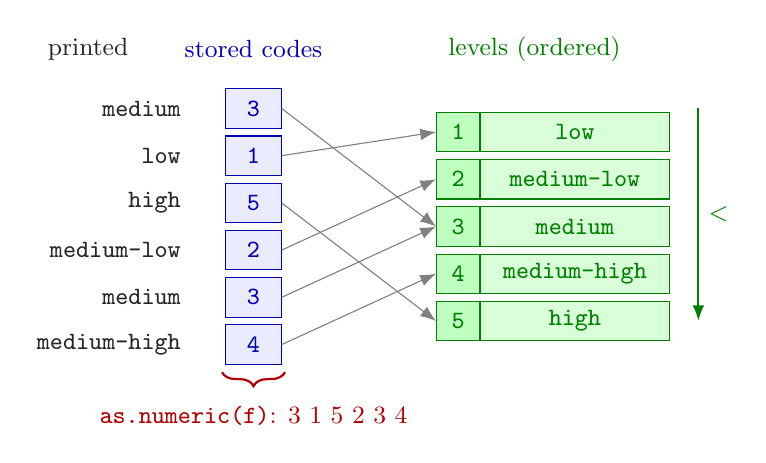
\begin{tikzpicture}[font=\small, >={Latex[length=2mm]},
  code/.style={draw=blue!70!black, fill=blue!8, text=blue!70!black, minimum width=0.7cm, minimum height=0.5cm, inner sep=1pt, font=\small\ttfamily},
  lvl/.style={draw=green!50!black, fill=green!15, text=green!50!black, minimum width=2.4cm, minimum height=0.5cm, inner sep=1pt, font=\small\ttfamily, anchor=west},
  lnum/.style={draw=green!50!black, fill=green!25, text=green!50!black, minimum width=0.55cm, minimum height=0.5cm, inner sep=1pt, font=\small\ttfamily}]
  % printed labels and stored codes
  \node[gray!30!black] at (0.3,0.75) {printed};
  \node[blue!70!black] at (2.4,0.75) {stored codes};
  \foreach \c/\l [count=\i] in {3/medium, 1/low, 5/high, 2/medium-low, 3/medium, 4/medium-high} {
    \node[font=\small\ttfamily, gray!30!black, anchor=east] at (1.6,-0.6*\i+0.6) {\l};
    \node[code] (c\i) at (2.4,-0.6*\i+0.6) {\c};
  }
  % levels
  \node[green!50!black, anchor=west] at (4.75,0.75) {levels (ordered)};
  \foreach \l [count=\j] in {low, medium-low, medium, medium-high, high} {
    \node[lnum] (n\j) at (5.0,-0.6*\j+0.3) {\j};
    \node[lvl] at (5.275,-0.6*\j+0.3) {\l};
  }
  \foreach \i/\c in {1/3, 2/1, 3/5, 4/2, 5/3, 6/4} { \draw[->, gray] (c\i.east) -- (n\c.west); }
  \draw[->, thick, green!50!black] (8.05,0.0) -- node[right, align=left] {$<$} (8.05,-2.7);
  % as.numeric
  \draw[decorate, decoration={brace, amplitude=5pt, mirror}, red!70!black, thick] (2.0,-3.35) -- (2.8,-3.35);
  \node[red!70!black, align=center] at (2.4,-3.9) {\texttt{as.numeric(f)}: 3 1 5 2 3 4};
\end{tikzpicture}
\end{document}
